%%=============================================================================
%%  The ModelSEED Biochemistry Database: 2026 update
%%  Target journal: Nucleic Acids Research (NAR), Database Issue
%%  https://academic.oup.com/nar/pages/Ms_Prep_Database
%%
%%  This is the ONLY file that carries journal formatting. All prose lives in
%%  sections/ and is pulled in by the \input statements at the bottom.
%%  Build:  pdflatex main -> bibtex main -> pdflatex main -> pdflatex main
%%          (or simply: latexmk -pdf main.tex)
%%=============================================================================

%%-----------------------------------------------------------------------------
%%  NAR DATABASE-ISSUE REQUIREMENTS CHECKLIST
%%  Summary only. The authoritative, fully-cited version -- including OUP's
%%  figure format/dpi specification -- is in NAR_REQUIREMENTS.md alongside
%%  this file. Update that file, not this comment.
%%  (from academic.oup.com/nar/pages/Ms_Prep_Database, checked 2026-08-26)
%%
%%  [ ] LENGTH -- update papers: normally no more than 4-6 typeset journal
%%      pages. Contact the Executive Editor before submitting anything longer.
%%      Current draft is deliberately over; trim after [TBD] markers resolve.
%%  [!] TITLE -- the database name should ideally be the FIRST WORD of the
%%      title. Current title opens with "The". Consider "ModelSEED Biochemistry
%%      Database, 2026 update: ..." to comply.
%%  [ ] URL -- a working URL must appear BOTH in the abstract and in the body.
%%      See \modelseedurl below; used in the abstract. The body carries the
%%      repository URL in sections/data_availability.tex.
%%  [ ] GRAPHICAL ABSTRACT -- MANDATORY. 5:2 aspect ratio, min 127x50 mm
%%      (5x2 in), TIF/EPS/editable PDF, 300-600 dpi, landscape, sans-serif
%%      (Arial) 12-16 pt. Must be ORIGINAL -- not reused from any main or
%%      supplementary figure. No trademarked/copyrighted logos.
%%      Submitted as a separate file, not embedded here.
%%  [ ] REFERENCES -- numbered sequentially in order of appearance. The class
%%      default (no namedate/numbered option) gives NAR-style numeric (1,2).
%%      Exclude "submitted"/"in preparation"/personal communications.
%%      Cite other databases by their most recent published description; if
%%      none exists, put the URL in body text, NOT in the reference list.
%%  [ ] FIGURES -- no numeric limit on figure count; the 4-6 page budget is the
%%      real constraint. The database home page may NOT be used as a typeset
%%      figure. A representative screenshot of a query result IS allowed.
%%      Format (OUP artwork guidance): raster -> uncompressed .tif; vector ->
%%      .eps/.svg/.pdf with embedded fonts. Minimum dpi: 300 colour half-tone,
%%      600 greyscale, 600-900 combination/line art, 1200 mono line art; vector
%%      has no inherent resolution. RGB preferred. Arial/Times/Courier/Symbol,
%%      text >= 7pt, lines 0.25-1pt. Prefer vector PDF/EPS from the figure
%%      scripts -- it sidesteps the dpi table entirely. See NAR_REQUIREMENTS.md.
%%  [ ] DATA AVAILABILITY -- must address formats and terms for data download.
%%  [ ] DATABASE ACCESS -- must be freely accessible without login; HTTPS
%%      encouraged; URL persistence expected for >= 5 years post-publication.
%%      Mobile/tablet accessibility is worth mentioning explicitly.
%%  [ ] INITIAL SUBMISSION -- one .pdf with main text, references, tables and
%%      figures EMBEDDED. Supplementary data as separate file(s). Number all
%%      pages (the class does this). Single-column/single-spaced is waived for
%%      LaTeX, so the two-column class output is correct as-is.
%%      DO NOT use line-numbering. DO NOT use footnotes. (Verified absent.)
%%  [ ] DISCLOSURES -- ORCID REQUIRED for the submitting author. Author
%%      Contributions statement MANDATORY (CRediT encouraged). Conflict of
%%      interest disclosure REQUIRED. AI assistance used in preparing this
%%      manuscript MUST be disclosed in the cover letter and in Methods or
%%      Acknowledgements. See NAR_REQUIREMENTS.md section 13.
%%  [ ] CODE DEPOSIT -- a GitHub URL is not sufficient; deposit to Zenodo or
%%      FigShare and put the permanent DOI in Data Availability at revision.
%%  [ ] SUBMISSION -- at least six suggested referees (name, institute, email),
%%      independent, not same institution/city as any author. Handled in
%%      ScholarOne at submission time, not in this file.
%%  [ ] DEADLINE -- update manuscripts due 15 September. Nothing before 1 June.
%%-----------------------------------------------------------------------------

%% NAR specifies the OUP template's "Modern Large" design -- do not change these
%% two options without checking NAR_REQUIREMENTS.md section 7 first.
%% Modern/large gives: 9bp body on 11.5pt leading, SANS-SERIF body text
%% (modern is the only one of the three designs that forces \sffamily),
%% 7.5bp footnotes, 210x276mm paper, two columns.
%% Other designs exist (contemporary|traditional x large|medium|mediumone|small)
%% but are not what NAR asks for.
%% Omitting namedate/numbered keeps the class default = numeric citations (NAR style).
\documentclass[unnumsec,webpdf,modern,large]{oup-authoring-template}

%\onecolumn  % uncomment for a wide single-column reading/review draft

%%-----------------------------------------------------------------------------
%%  NAR revision markup: the referee-facing "marked" copy is now generated by
%%  running latexdiff between the pre-PR-297 and post-PR-297 versions of this
%%  file (see Papers/NAR_Update_2026/latex/README or the PR description for
%%  the exact command). No in-source markup macro is needed any more.
%%-----------------------------------------------------------------------------

%%-----------------------------------------------------------------------------
%%  Packages. The class already loads: amsmath, amssymb, graphicx, hyperref,
%%  natbib, array, multirow, xcolor, tikz, url, caption, rotating, listings.
%%  It also defines \toprule / \midrule / \botrule itself -- do NOT load
%%  booktabs, it clashes.
%%-----------------------------------------------------------------------------
%% NOTE: the OUP manual asks authors to "refrain from adding further packages
%% or macros if possible", so nothing is loaded here. The draft-marker and
%% domain-shorthand macros below are the only additions, and the markers
%% disappear entirely under \draftmodefalse.

%%-----------------------------------------------------------------------------
%%  Draft markers.
%%  The source manuscript carries [TBD] and [DRAFT PENDING] placeholders.
%%  They are rendered in colour while drafting so they are impossible to miss.
%%  Flip \draftmodefalse (or pass \draftmodefalse before \begin{document})
%%  to make every marker vanish for a clean submission PDF.
%%-----------------------------------------------------------------------------
\newif\ifdraftmode
\draftmodetrue          % <-- set to \draftmodefalse for the submission build

\ifdraftmode
  \newcommand{\TBD}[1][]{\textcolor{red}{\textbf{[TBD}\ifx\relax#1\relax\else\ #1\fi\textbf{]}}}
  \newcommand{\DRAFTPENDING}[1]{\textcolor{orange}{\textbf{[DRAFT PENDING]}\ --\ #1}}
  \newcommand{\NUMBERSPENDING}[1]{\textcolor{orange}{\textbf{[NUMBERS PENDING]}\ #1}}
\else
  \newcommand{\TBD}[1][]{}
  \newcommand{\DRAFTPENDING}[1]{}
  \newcommand{\NUMBERSPENDING}[1]{}
\fi

%%-----------------------------------------------------------------------------
%%  Domain shorthands. Greek in text mode is unreliable under pdflatex, so all
%%  thermodynamic symbols route through math mode here.
%%-----------------------------------------------------------------------------
\newcommand{\dfG}{$\Delta_{\mathrm{f}}G'$}          % formation energy
\newcommand{\drG}{$\Delta_{\mathrm{r}}G'$}          % reaction energy
\newcommand{\drGo}{$\Delta_{\mathrm{r}}G'^{\circ}$} % standard reaction energy
\newcommand{\modelseedurl}{\url{https://modelseed.org}}
\newcommand{\repourl}{\url{https://github.com/ModelSEED/ModelSEEDDatabase}}
\newcommand{\file}[1]{\texttt{#1}}                  % repo paths / filenames
\newcommand{\cpd}[1]{\texttt{#1}}                   % compound identifiers

%% The OUP class sets \flushbottom (cls line 2513). With a short column the
%% slack is absorbed by the most elastic glue on the page -- the space above
%% \subsection headings -- which opened visible gaps before 'Atom mapping'
%% and 'Distribution and community process'. \raggedbottom lets a column end
%% short instead. Standard LaTeX, no package and no class option.
\raggedbottom
%DIF PREAMBLE EXTENSION ADDED BY LATEXDIFF
%DIF UNDERLINE PREAMBLE %DIF PREAMBLE
\RequirePackage[normalem]{ulem} %DIF PREAMBLE
\RequirePackage{color}\definecolor{RED}{rgb}{1,0,0}\definecolor{BLUE}{rgb}{0,0,1} %DIF PREAMBLE
\providecommand{\DIFadd}[1]{{\protect\color{red}{#1}}} %DIF PREAMBLE
\providecommand{\DIFdel}[1]{{\protect\color{red}\sout{#1}}} %DIF PREAMBLE
%DIF SAFE PREAMBLE %DIF PREAMBLE
\providecommand{\DIFaddbegin}{} %DIF PREAMBLE
\providecommand{\DIFaddend}{} %DIF PREAMBLE
\providecommand{\DIFdelbegin}{} %DIF PREAMBLE
\providecommand{\DIFdelend}{} %DIF PREAMBLE
\providecommand{\DIFmodbegin}{} %DIF PREAMBLE
\providecommand{\DIFmodend}{} %DIF PREAMBLE
%DIF FLOATSAFE PREAMBLE %DIF PREAMBLE
\providecommand{\DIFaddFL}[1]{\DIFadd{#1}} %DIF PREAMBLE
\providecommand{\DIFdelFL}[1]{\DIFdel{#1}} %DIF PREAMBLE
\providecommand{\DIFaddbeginFL}{} %DIF PREAMBLE
\providecommand{\DIFaddendFL}{} %DIF PREAMBLE
\providecommand{\DIFdelbeginFL}{} %DIF PREAMBLE
\providecommand{\DIFdelendFL}{} %DIF PREAMBLE
%DIF COLORLISTINGS PREAMBLE %DIF PREAMBLE
\RequirePackage{listings} %DIF PREAMBLE
\RequirePackage{color} %DIF PREAMBLE
\lstdefinelanguage{DIFcode}{ %DIF PREAMBLE
%DIF DIFCODE_UNDERLINE %DIF PREAMBLE
  moredelim=[il][\color{red}\sout]{\%DIF\ <\ }, %DIF PREAMBLE
  moredelim=[il][\color{blue}\uwave]{\%DIF\ >\ } %DIF PREAMBLE
} %DIF PREAMBLE
\lstdefinestyle{DIFverbatimstyle}{ %DIF PREAMBLE
	language=DIFcode, %DIF PREAMBLE
	basicstyle=\ttfamily, %DIF PREAMBLE
	columns=fullflexible, %DIF PREAMBLE
	keepspaces=true %DIF PREAMBLE
} %DIF PREAMBLE
\lstnewenvironment{DIFverbatim}[1][]{\lstset{style=DIFverbatimstyle}}{} %DIF PREAMBLE
\lstnewenvironment{DIFverbatim*}[1][]{\lstset{style=DIFverbatimstyle,showspaces=true}}{} %DIF PREAMBLE
\lstset{extendedchars=\true,inputencoding=utf8}

%DIF END PREAMBLE EXTENSION ADDED BY LATEXDIFF

\begin{document}

%%-----------------------------------------------------------------------------
%%  Journal metadata -- production fills most of this in.
%%-----------------------------------------------------------------------------
%% The class calls \societylogo{} in the running head but leaves every
%% definition commented out (oup-authoring-template.cls:921-926), so it is
%% undefined unless the author supplies one. NAR is not a society journal with
%% a logo here, so the empty form the class itself offers is used. Without this
%% every build raised "Undefined control sequence" plus three "Missing number"
%% errors and still produced a PDF, which is why it went unnoticed.
\def\societylogo{}%
%% Journal identity is switched off for the bioRxiv build. preprint.tex
%% compiles this same file a second time with \PREPRINTBUILD defined, so the
%% preprint carries no NAR or OUP identity for a paper the journal has not
%% accepted. The \else branch is the NAR submission and is unchanged.
\ifdefined\PREPRINTBUILD
  \journaltitle{}
  \DOI{}
  \copyrightyear{2026}
  \pubyear{2026}
  \vol{}
  \issue{}
  \access{}
  \appnotes{}
  %% Blanking the metadata empties the strings but leaves the running head's
  %% punctuation skeleton (", 2026, Volume , Issue"), and the title-page band
  %% still draws its rule and logo box. Both page styles are therefore replaced
  %% outright with a bare folio. Defined after \documentclass, so these override
  %% the class definitions at lines 870 and 928.
  \makeatletter
  \def\ps@headings{%
    \def\@oddhead{\hfill{\sffamily\fontsize{9bp}{11bp}\selectfont\thepage}}%
    \def\@evenhead{{\sffamily\fontsize{9bp}{11bp}\selectfont\thepage}\hfill}%
    \def\@oddfoot{}\def\@evenfoot{}}
  \def\ps@opening{%
    \def\@oddhead{}\def\@evenhead{}\def\@oddfoot{}\def\@evenfoot{}}
  %% The class EXECUTES \ps@headings at load time (cls line 2515), so \@oddhead
  %% was already fixed before the redefinition above. Re-invoke it to install
  %% the new one. \ps@opening needs no such call: \maketitle reaches it later
  %% through \thispagestyle{opening}.
  \ps@headings
  \makeatother
\else
  \journaltitle{Nucleic Acids Research}
  \DOI{DOI added during production}
  \copyrightyear{2026}
  \pubyear{2026}
  \vol{00}
  \issue{0}
  \access{Advance Access Publication Date: Day Month Year}
  \appnotes{Database Issue}
\fi

\firstpage{1}
%% \lastpage must be set too. Unset, the class falls through \setlastpage to
%% its aux-file path, hands \relax to \@arabic and throws three "Missing
%% number, treated as zero" errors on every page shipout while still producing
%% a PDF. Update if the page count changes; production overwrites both.
\lastpage{6}

%\subtitle{Database Issue}

%%-----------------------------------------------------------------------------
%%  Title
%%  NAR: the database name should ideally be the first word. See checklist.
%%-----------------------------------------------------------------------------
%% Shortened 2026-09-15. The previous title's last clause -- "the impact of
%% reaction-direction assignments on metabolic-model output" -- promised an
%% analysis the paper does not contain: no section reports model output, flux
%% or biomass. Do not reinstate it without the analysis.
\title[ModelSEED Biochemistry Database, 2026 update]{The ModelSEED Biochemistry
Database, 2026 update: grading multi-source thermodynamics}

%%-----------------------------------------------------------------------------
%%  Authors
%%  \TBD -- the 2020 author list plus this cycle's contributors, minus anyone
%%  stepping off, in the agreed order. See PAPER_2026_PLAN.md open decision #3
%%  (untracked; local to the author's tree, not in the repository)
%%  for the Nikoloski-lab crediting format.
%%-----------------------------------------------------------------------------
%% ORCID is REQUIRED for the submitting author (NAR_REQUIREMENTS.md section 13).
%% Attach with \ORCID{0000-0000-0000-0000} directly after the author name.
%% AUTHOR LIST, per Sam 2026-09-07. Order: lead, then Argonne/Henry team with
%% the two interns, then the upstream-tool contributors grouped by tool, then
%% the KBase PIs, then the two corresponding authors last.
%%
%% SPELLINGS VERIFIED against published records, not transcribed. Five were
%% corrected from the names as first given:
%%   Beber      not "Bieber"    -- references.bib beber2022, and Seaver 2020
%%   Giessmann  not "Greissman" -- 10.3762/bjoc.19.26, IGDORE Berlin
%%   Setlur     not "Setler"    -- his fork, github.com/VibhavSetlur
%%   Wood-Charlson, Elisha M.   -- given only as "Elisha"; Seaver 2020
%%   Anand, Mohit               -- the third Maranas-lab author, 10.1371/journal.pcbi.1012516
%%                                 (novoStoic2.0, with Upadhyay and Maranas)
%% Faria, Edirisinghe, Liu, Arkin, Cottingham, Henry, Seaver all confirmed
%% against Seaver et al. 2020 (10.1093/nar/gkaa746).
%%
%% ORCIDs. Seven are CONFIRMED FROM A PUBLICATION -- the author list of
%% Seaver et al. 2020, read through Europe PMC's core result type, which
%% embeds ORCIDs per author:
%%   https://www.ebi.ac.uk/europepmc/webservices/rest/search?query=EXT_ID:32986834&resultType=core&format=json
%% Seaver's also cross-validates against the ORCID public API by name search,
%% which is the other reliable route:
%%   https://pub.orcid.org/v3.0/expanded-search/?q=family-name:X+AND+given-names:Y
%% Publisher pages are NOT a usable source: sciencedirect.com returns 403 to
%% automated fetches, as do AIP, RSC and ACS.
%%
%% Henry's ORCID 0000-0001-8058-9123 was confirmed by Chris himself
%% (2026-09-15), along with chenry@anl.gov. It is no longer inferred.
%%
%% STILL MISSING: Freiburger, Faria, Taylor, Setlur, Upadhyay, Anand, Maranas,
%% Giessmann, Wood-Charlson. Faria and Wood-Charlson carry no ORCID in either
%% paper checked, so those must come from the people themselves.
%%
%% AFFILIATION 9 (Penn State) is confirmed against MechFind, Nat Commun 2026,
%% 10.1038/s41467-026-71957-0 (PMID 42056099), where Maranas is corresponding
%% author at exactly this address -- Department of Chemical Engineering, The
%% Pennsylvania State University, University Park, PA 16802 -- matching the
%% string below character for character. Retrieved via PubMed 2026-09-15.
%%
%% Two caveats. Maranas ALSO lists "The Center for Bioenergy Innovation, Oak
%% Ridge, TN 37830" as a second affiliation on that paper; we carry only the
%% Penn State one, per Sam. And Anand is NOT an author on MechFind, so his
%% Penn State affiliation is still inferred -- from novoStoic2.0
%% (10.1371/journal.pcbi.1012516) and from sharing Maranas's lab. Upadhyay is
%% listed at Penn State on MechFind too but has since moved to Illinois and
%% told us so himself, which is the standing reason to treat a lab-mate's
%% published affiliation as a starting point rather than an answer.
%%
 %DIF > % Numbering below runs in order of first appearance, except [14], [15] and
%DIF > % [16], added 2026-10 for Zhu, Ramanathan and Freiburger's second
%DIF > % affiliation after the original list was fixed -- appending rather than
%DIF > % renumbering 1-13 to avoid touching every other author's citation.
\DIFaddbegin \author[1,16]{\DIFaddend Andrew Freiburger\ORCID{0000-0002-7288-535X}}
\author[1]{Jos\'e P. Faria\ORCID{0000-0001-9302-7250}}
\DIFaddbegin \author[1,14]{\DIFadd{Ray Zhu}\ORCID{0000-0001-9316-7245}}
\DIFaddend \author[1]{Janaka N. Edirisinghe\ORCID{0000-0003-2493-234X}}
\author[1]{Filipe Liu\ORCID{0000-0001-8701-2984}}
\author[2]{Cooper Taylor\ORCID{0009-0003-2147-1960}}
\author[1]{Vibhav Setlur\ORCID{0009-0000-6823-9761}}
\author[3,4]{Robert T. Giessmann}
\author[5]{Moritz E. Beber\ORCID{0000-0003-2406-1978}}
\author[6]{Elad Noor\ORCID{0000-0001-8776-4799}}
\author[7,8]{Vikas Upadhyay\ORCID{0000-0003-2266-5073}}
\author[9]{Mohit Anand}
\author[9]{Costas D. Maranas}
\author[10,11]{Sebastian Hu{\ss}\ORCID{0000-0003-0712-2986}}
\author[10,11]{Zoran Nikoloski\ORCID{0000-0003-2671-6763}}
\author[12]{Adam P. Arkin\ORCID{0000-0002-4999-2931}}
\author[13]{Robert W. Cottingham\ORCID{0000-0002-2775-3905}}
\author[12]{Elisha M. Wood-Charlson\ORCID{0000-0001-9557-7715}}
\DIFaddbegin \author[1,15]{\DIFadd{Arvind Ramanathan}\ORCID{0000-0002-1622-5488}}
\DIFaddend \author[1,$\dagger$]{Christopher S. Henry\ORCID{0000-0001-8058-9123}}
\author[1,$\ast$]{Samuel M. D. Seaver\ORCID{0000-0002-7674-5194}}

\address[1]{\orgdiv{Division of Data Science and Learning},
\orgname{Argonne National Laboratory}, \orgaddress{\street{9700 S. Cass Ave.},
\postcode{60439}, \state{Lemont, IL}, \country{USA}}}

%% 2 supplied by Sam (2026-09-11) on Cooper Taylor moving from Argonne. No
%% postcode given, so none is written -- every other address here carries one.
\address[2]{\orgdiv{College of Engineering, Computing and Applied Sciences},
\orgname{Clemson University},
\orgaddress{\state{Clemson, SC}, \country{USA}}}

\address[3]{\orgname{Institute for Globally Distributed Open Research and Education (IGDORE)},
\orgaddress{\state{Berlin}, \country{Germany}}}

\address[4]{\orgdiv{Faculty II Mathematics and Natural Sciences, Institute of Chemistry, Chair of Biochemistry of Gas-Converting Biocatalysts},
\orgname{Technische Universit\"at Berlin},
\orgaddress{\state{Berlin}, \country{Germany}}}

\address[5]{\orgname{Institute for Globally Distributed Open Research and Education (IGDORE)},
\orgaddress{\state{Copenhagen}, \country{Denmark}}}

\address[6]{\orgdiv{Department of Plant and Environmental Sciences},
\orgname{Weizmann Institute of Science},
\orgaddress{\state{Rehovot}, \country{Israel}}}

%% 7 and 8 supplied by Vikas Upadhyay himself (2026-09-10) on moving from
%% Penn State; contact viku@illinois.edu. He holds both.
\address[7]{\orgdiv{NSF iBioFoundry},
\orgname{University of Illinois Urbana-Champaign},
\orgaddress{\postcode{61801}, \state{Urbana, IL}, \country{USA}}}

\address[8]{\orgdiv{Carl R. Woese Institute for Genomic Biology},
\orgname{University of Illinois Urbana-Champaign},
\orgaddress{\postcode{61801}, \state{Urbana, IL}, \country{USA}}}

\address[9]{\orgdiv{Department of Chemical Engineering},
\orgname{The Pennsylvania State University},
\orgaddress{\postcode{16802}, \state{University Park, PA}, \country{USA}}}

%% 10 and 11 are transcribed from Hu{\ss} et al. 2022 (10.1111/tpj.15903) via
%% Crossref, so they are 2022-vintage and unconfirmed by Hu{\ss} or Nikoloski:
%% confirm with them before submission.
\address[10]{\orgdiv{Systems Biology and Mathematical Modelling Group},
\orgname{Max Planck Institute of Molecular Plant Physiology},
\orgaddress{\street{Am M\"uhlenberg 1}, \postcode{14476}, \state{Potsdam},
\country{Germany}}}

\address[11]{\orgdiv{Bioinformatics, Institute of Biochemistry and Biology},
\orgname{University of Potsdam},
\orgaddress{\street{Karl-Liebknecht-Str. 24-25}, \postcode{14476},
\state{Potsdam}, \country{Germany}}}

\address[12]{\orgdiv{Environmental Genomics and Systems Biology Division},
\orgname{Lawrence Berkeley National Laboratory},
\orgaddress{\postcode{94720}, \state{Berkeley, CA}, \country{USA}}}

\address[13]{\orgdiv{Biosciences Division},
\orgname{Oak Ridge National Laboratory},
\orgaddress{\postcode{37830}, \state{Oak Ridge, TN}, \country{USA}}}

%DIF > % 14 supplied by Ray Zhu directly (2026-10), including his own correction
%DIF > % adding the DSL/Argonne affiliation he first omitted -- hence Zhu also
%DIF > % carrying [1] above, not just [14].
\DIFaddbegin \address[14]{\orgdiv{Pritzker School of Molecular Engineering},
\orgname{University of Chicago},
\orgaddress{\state{Hyde Park, IL}, \country{USA}}}

%DIF > % 15 supplied for Arvind Ramanathan (2026-10); he holds both the Argonne DSL
%DIF > % appointment (already [1] above) and this University of Chicago one.
\address[15]{\orgdiv{Consortium for Advanced Science and Engineering},
\orgname{University of Chicago},
\orgaddress{\state{Hyde Park, IL}, \country{USA}}}

%DIF > % 16 supplied for Andrew Freiburger (2026-10); he holds both the Argonne DSL
%DIF > % appointment (already [1] above) and this Northwestern one.
\address[16]{\orgdiv{Department of Chemical and Biological Engineering},
\orgname{Northwestern University},
\orgaddress{\state{Evanston, IL}, \country{USA}}}

\DIFaddend \corresp[$\ast$]{Corresponding author. \href{mailto:seaver@anl.gov}{seaver@anl.gov}}
\corresp[$\dagger$]{Corresponding author. \href{mailto:chenry@anl.gov}{chenry@anl.gov}}

%% Submission history. Left commented out deliberately: the month argument is
%% fed to \numexpr by the class (\myswitch, cls:1175), so an empty
%% \received{}{}{} throws "Missing number, treated as zero" -- once per macro --
%% while still producing a PDF. These dates are not knowable before submission
%% and are set by production. To use them, give a NUMERIC month:
%%   \received{1}{9}{2026}
%\received{}{}{}
%\revised{}{}{}
%\accepted{}{}{}

%%-----------------------------------------------------------------------------
%%  Abstract -- must contain a working URL (NAR requirement).
%%  Abstracts must stand alone: no citations to the reference list, no
%%  equations, no cross-references.
%%-----------------------------------------------------------------------------
 \DIFaddbegin \abstract{%% NAR: must contain a working URL; must stand alone (no citations, no
%% equations, no cross-references); keep as a SINGLE paragraph -- it is
%% \input into the \abstract{} argument in main.tex.
%%
%% Rewritten 2026-09-05 to the 6-page shape. Every number here is measured and
%% appears in the Results. Deliberately omitted, because the sections that
%% carried them are now Supplementary: PubChem validation, protein-carrier
%% cofactor standardisation, the reaction-similarity foundation model, and the
%% v2 draft-model direction-sensitivity study, which is not yet run.
The ModelSEED Biochemistry Database (\modelseedurl) supplies foundational mass- and charge-balanced reaction networks for metabolic reconstructions.
Here we present an update on the biochemistry where the database has been expanded to $\sim46,000$ compounds, featuring $\sim37,000$ metabolic structures, and $\sim48,000$ reactions.
We expanded our approach for handling thermodynamic data, enabling multiple sources of data to be derived, integrated, and presented to the wider research community.
We now publish predictions of pKa, reaction energy (and respective uncertainties), and estimates of reaction direction from multiple independent sources.
Reaction directions are graded gold, silver, or bronze according to the strength of supporting evidence, which is complemented by the prediction from an ensemble of large language models.
These diverse sources empower users to understand agreements or discrepancies in directionality for $\sim27,000$ reactions.
Finally, to ensure data integrity, a new conflict-resolution pipeline reconciles structures across sources, documenting input from curators.
Our work is publicly available at \url{https://github.com/ModelSEED/ModelSEEDDatabase}.
}
\DIFaddend 

\keywords{biochemistry database, metabolic modelling, thermodynamics,
reaction reversibility, ModelSEED}

\maketitle

%%=============================================================================
%%  BODY -- every section below is a separate file in sections/.
%%  Reorder, comment out, or add \input lines here; do not put prose in
%%  this file.
%%=============================================================================

%DIF > % Figure 1 is declared here (moved from M06, 2026-10) so that LaTeX places it
%DIF > % at the top of page 2. A float cannot move backwards past its declaration,
%DIF > % so the position of this block IS the page choice -- Figures 2 and 3 are
%DIF > % positioned the same way, in M11 and M12 respectively, for pages 3 and 4.
%DIF > % \ref{fig:growth} still resolves from M09, where the figure is discussed.
\DIFaddbegin \begin{figure*}[!t] \centerline{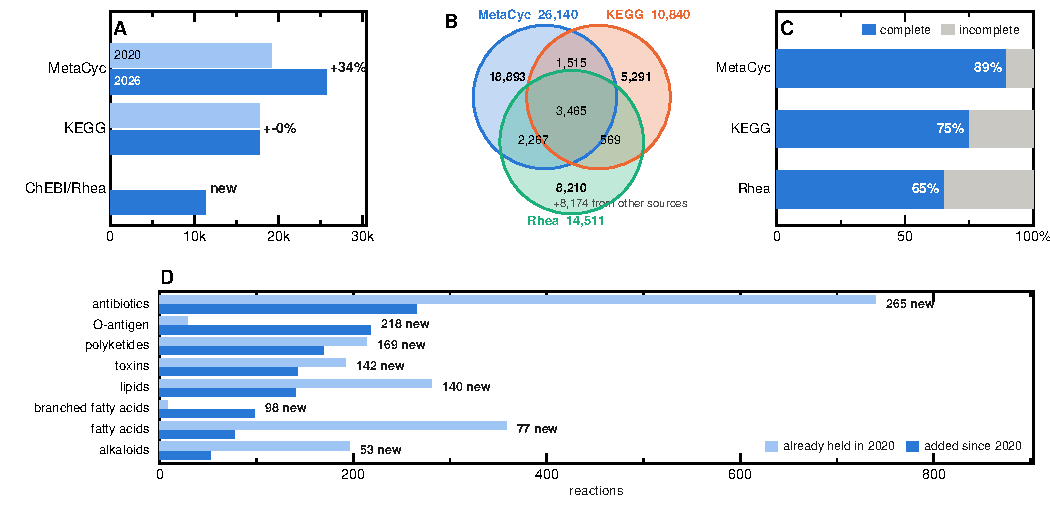
\includegraphics[width=\textwidth]{../figures/figure1_growth.pdf}} \caption{\textbf{\DIFaddFL{Sources of compounds and reactions.}} \DIFaddFL{(}\textbf{\DIFaddFL{A}}\DIFaddFL{) compounds contributed by each source that also supplied molecular structures, 2020 against 2026: we did not introduce any new biochemistry from KEGG. The third row is ChEBI, which supplies structures but no reactions. (}\textbf{\DIFaddFL{B}}\DIFaddFL{) how the three primary reaction sources overlap, every region labelled with its reaction count. Circle areas are not proportional. Rhea identifies its compounds through ChEBI. (}\textbf{\DIFaddFL{C}}\DIFaddFL{) the share of each source's unique reactions that are complete, meaning every reagent is assigned a complete structure, so the reaction can be balanced and decomposed.}} \label{fig:growth} \end{figure*}

\DIFaddend \section{Introduction}


The ModelSEED Biochemistry Database provides mass- and charge-balanced reaction networks reconciled across major biochemical resources for metabolic reconstructions~\cite{seaver2020}.
Since its 2020 release, the database has been widely adopted for \DIFaddbegin \DIFadd{curating }\DIFaddend genome-scale metabolic  \DIFaddbegin \DIFadd{models (GEMs): e.g. GEMsembler utilizes it for cross-mapping between resources~\mbox{%DIFAUXCMD
\cite{gemsembler2025} }\hskip0pt%DIFAUXCMD
}\DIFaddend and Yeast9  \DIFaddbegin \DIFadd{sources Gibbs energies from it for constraining the core GEM}\DIFaddend ~\cite{yeast9}.
 This update reports  \DIFaddbegin \DIFadd{an expansion }\DIFaddend of the database,  \DIFaddbegin \DIFadd{a tiered integration of thermodynamic sources spanning heuristic methods to large language models, and graded confidence scores for reaction directionality based on supporting evidence.
While $>70\%$ of sources }\DIFaddend agree on reaction  \DIFaddbegin \DIFadd{directionality, disagreements are displayed for investigators to interpret.
Atom-mapping data is further integrated to enable metabolic flux analysis (MFA)}\DIFaddend , and a structure-curation pipeline \DIFaddbegin \DIFadd{is }\DIFaddend built to resolve  \DIFaddbegin \DIFadd{conflicts }\DIFaddend between structures from different databases.
Finally, we expanded our search interface at https://modelseed.org \DIFaddbegin \DIFadd{/biochem to facilitate user queries of the resource}\DIFaddend .

\section{Materials and Methods}
%% Consolidates the former methods_{collation,integration,provenance,transport,
\subsection{Construction and Curation}\label{sec:methods-construction}

We collated additional compounds and reactions from MetaCyc~\cite{caspi2020}, Rhea~\cite{bansal2022}, and ChEBI~\cite{hastings2016} \DIFaddbegin \DIFadd{, merging compounds via }\DIFaddend structures where possible and  \DIFaddbegin \DIFadd{matching reactions by compound identities, similar to the }\DIFaddend 2020 release~\cite{seaver2020}.
Mass and charge  \DIFaddbegin \DIFadd{balances are }\DIFaddend enforced and flagged.
 \DIFaddbegin \DIFadd{Unlike }\DIFaddend the 2020 release,  \DIFaddbegin \DIFadd{where compounds with conflicting sourced structures were }\DIFaddend either manually reviewed or  \DIFaddbegin \DIFadd{silently dropped, the }\DIFaddend updated pipeline classifies  \DIFaddbegin \DIFadd{structural conflicts and either 1) automatically picks }\DIFaddend from the source  \DIFaddbegin \DIFadd{that matches }\DIFaddend the historical formula,  \DIFaddbegin \DIFadd{2) prioritizes curator authored and justified content, or 3) excludes (with logged justification) compounds without a defensible source formula.
This enforces that every }\DIFaddend outcome is attributed to its curator and  \DIFaddbegin \DIFadd{evidence.
Every structure is retained }\DIFaddend in the repository  \DIFaddbegin \DIFadd{to facilitate conflict resolution.
Investigators can contribute to the ModelSEED Database through the procedure }\DIFaddend in Supplementary Methods~S1 \DIFaddbegin \DIFadd{, which is }\DIFaddend expanded in the repository.
%DIF > % Figure 2 is declared here (moved 2026-10) so that LaTeX places it at the
%DIF > % top of page 3; see M02's comment on Figure 1 for the scheme. (Declaring it
%DIF > % any earlier, e.g. in M03, lets it stack onto page 2 alongside Figure 1
%DIF > % instead.)
\DIFaddbegin \begin{figure*}[!t]
    \centerline{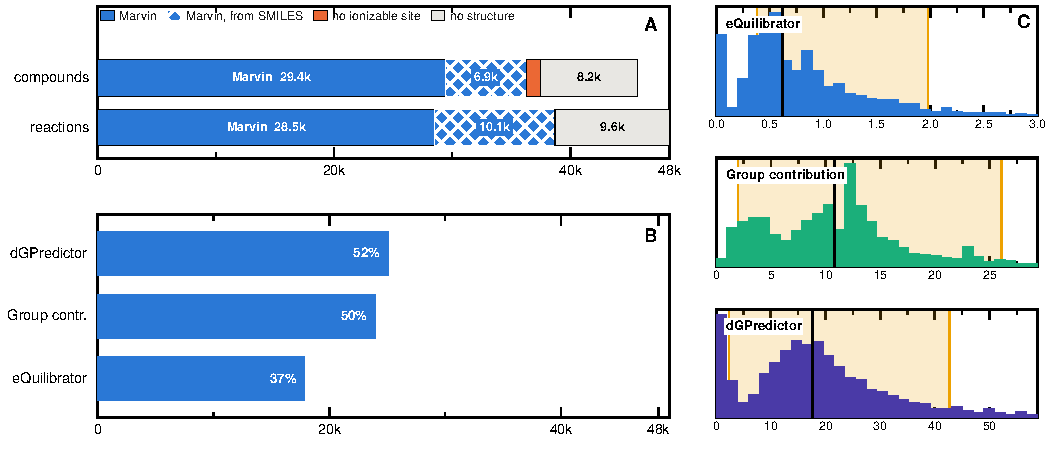
\includegraphics[width=\textwidth]{../figures/figure2_thermodynamics.pdf}}
    \caption{
        \textbf{\DIFaddFL{Thermodynamic sources.}} \DIFaddFL{(}\textbf{\DIFaddFL{A}}\DIFaddFL{) Provenance of every pK$_\mathrm{a}$ ladder shipped in the database, across all 45,662 compounds and 48,384 reactions. ChemAxon Marvin supplies 79.4\% of compounds and 79.8\% of reactions. }\emph{\DIFaddFL{Hatching}} \DIFaddFL{marks the share computed from SMILES because Marvin refuses polymers and organometallics as query molecules. }\emph{\DIFaddFL{No ionizable site}} \DIFaddFL{edscribes 1,237 compounds that lacked a dissociable proton from Marvin between pH $-2$ and $16$. (}\textbf{\DIFaddFL{B}}\DIFaddFL{) Reactions that carry an energy computed from the source heuristic. (}\textbf{\DIFaddFL{C}}\DIFaddFL{) Reported uncertainties (kcal\,mol$^{-1}$) for each source, where the shaded band spans the 5th to 95th percentile range used in our classification scheme.
        }}
    \label{fig:thermo}
\end{figure*}

\DIFaddend %% Rewritten 2026-09-08 after the Marvin 26.1 regeneration and the reversibility
%% overhaul. Every number here is measured against the shipped files; see the
%% inline comments for the command that reproduces each. Detail in
%% Supplementary Methods S2.
\subsection{Multi-source thermodynamics}\label{sec:methods-thermo}

The 2020 release combined two  \DIFaddbegin \DIFadd{thermodynamics sources: eQuilibrator~\mbox{%DIFAUXCMD
\cite{flamholz2012} }\hskip0pt%DIFAUXCMD
and the group contribution method~\mbox{%DIFAUXCMD
\cite{jankowski2008}}\hskip0pt%DIFAUXCMD
.
This ModelSEED Database update incorporates the most recent }\DIFaddend eQuilibrator~3.0~\cite{beber2022}  \DIFaddbegin \DIFadd{and introduces two new thermodynamics sources: }\DIFaddend dGPredictor~\cite{wang2021}  and experimental values .
\DIFaddbegin \DIFadd{Each of these four distinct thermodynamics sources are reported separately where available.
}\DIFaddend All values are reported at pH~7.0, ionic strength 0.25\,M, pMg~3.0 and 298.15\,K; the basis for each condition and its effect on the released energies are given in Supplementary Methods~S2.

\paragraph{Protonation.} eQuilibrator's Legendre transform requires a \emph{macroscopic} pKa ladder per compound: an ordered list in which consecutive species differ by one proton.
The count of entries around the desired pH sets the proton count of the major microspecies, so the composition of the ladder changes the transformed energy directly.
We generate the pKa ladders  \DIFaddbegin \DIFadd{for }\DIFaddend every compound with a structure \DIFaddbegin \DIFadd{(source prevenance preserved)}\DIFaddend , and the measured ladders of Alberty~\cite{alberty2003},  \DIFaddbegin \DIFadd{using licensed ChemAxon Marvin 26.1~\mbox{%DIFAUXCMD
\cite{marvin} }\hskip0pt%DIFAUXCMD
for use with eQuilibrator and also via open-source MolGpKa~\mbox{%DIFAUXCMD
\cite{pan2021} }\hskip0pt%DIFAUXCMD
for unlicensed use}\DIFaddend . 

\paragraph{Experimental anchors.} eQuilibrator and dGPredictor draw on the same set of experimental values derived from the NIST Thermodynamics of Enzyme-catalyzed Reactions (TECR) Database~\cite{goldberg2004} \DIFaddbegin \DIFadd{.
There were structural conflicts in compounds mapped to ModelSEED from the KEGG IDs of TECR and the MetaNetX IDs of eQuilibrator, so to facilitate direct comparisons between thermodynamic predictions of ModelSEED reactions, we }\DIFaddend re-built the experimental anchors of TECR values  \DIFaddbegin \DIFadd{and curated conflicts to map TECR directly to ModelSEED.
We further investigated }\DIFaddend openTECR, a communal re-curation of  \DIFaddbegin \DIFadd{TECR available at }\DIFaddend \url{https://github.com/opentecr} , to extend the  \DIFaddbegin \DIFadd{thermodynamic }\DIFaddend anchors.

 \paragraph{Direction.}  \DIFaddbegin \DIFadd{To conserve precedence}\DIFaddend , we use the same  \DIFaddbegin \DIFadd{2020 heuristics to derive reaction directions }\DIFaddend from the Group contribution approach~\cite{jankowski2008} , so that series stays comparable across releases.
For eQuilibrator and dGPredictor\DIFaddbegin \DIFadd{, }\DIFaddend we use one rule set built on the reversibility index from Noor \textit{et al.}~\cite{noor2012}:  irreversible when $|\ln\Gamma|$ exceeds $\ln(1000)$ by more than one propagated standard deviation~\cite{beber2022}, \DIFaddbegin \DIFadd{where }\DIFaddend $\Gamma$  \DIFaddbegin \DIFadd{is }\DIFaddend the fold-change of reactant concentration required to change reaction direction \DIFaddbegin \DIFadd{.
We extend the rule to require that the uncertainty clears this $\Gamma$ }\DIFaddend threshold as well \DIFaddbegin \DIFadd{; however, differences in how each source estimates its uncertainty prevent direct comparisons (Figure~\ref{fig:thermo}C)).
%DIF > % Figure 1 moved to M02 (2026-10) to pull it onto page 2; see M02's own
%DIF > % comment for the current page-placement scheme.
}\DIFaddend %% Compact Methods statement for BOTH routes to a direction claim. The full
%% specification of each lives in the supplement:
%%   grading  -> Supplementary Methods S3
%%   ensemble -> Supplementary Methods S4
%% Do not re-expand either here; the budget is 4-6 typeset pages and the detail
%% was moved out deliberately.
\subsection{Grading reaction direction}\label{sec:methods-grading}

We apply a classification approach with which we grade the predicted reaction direction based on the \DIFaddbegin \DIFadd{quality of }\DIFaddend available evidence.
 \DIFaddbegin \DIFadd{The selected tiers are intuitively described as gold (highest), silver (intermediate)}\DIFaddend ,  or bronze \DIFaddbegin \DIFadd{(lowest)}\DIFaddend .
Our evaluation splits two ways \DIFaddbegin \DIFadd{: 1) }\DIFaddend confidence of a source's own claim  \DIFaddbegin \DIFadd{fit }\DIFaddend as a probability against the experimental anchors  \DIFaddbegin \DIFadd{and 2) }\DIFaddend a weighted comparison \DIFaddbegin \DIFadd{of other sources }\DIFaddend on the same scale.
Grades, self-assessments, and cross-source verdicts are stored in the biochemistry database  \DIFaddbegin \DIFadd{and exposed on the website for users inspection.
The grading methodology is thoroughly described }\DIFaddend in Supplementary Methods~S3.

\subsection{Ensemble LLMs predictions}\label{sec:llm-grading}
Thermodynamic assignment is bounded by estimate coverage \DIFaddbegin \DIFadd{, which means that energies and therefore directions }\DIFaddend cannot be computed for  23,790  \DIFaddbegin \DIFadd{structurally incomplete reactions.
We therefore }\DIFaddend run a complementary approach using an ensemble  \DIFaddbegin \DIFadd{or "council" }\DIFaddend of large language models (LLMs) to  \DIFaddbegin \DIFadd{estimate directionality from only reaction }\DIFaddend name and stoichiometry \DIFaddbegin \DIFadd{, where three LLM agents independently predict a direction}\DIFaddend , a fourth audits, and a fifth adjudicates.
We provide the prompts in the repository, and describe the process and its  \DIFaddbegin \DIFadd{limitations }\DIFaddend in Supplementary Methods~S4.
 %% Consolidates the former methods_{reaction_similarity,atom_mapping} sections.
\subsection{Atom mapping}\label{sec:methods-mapping}

Atom mappings are generated from the workflow of Hu{\ss} \textit{et al.}~\cite{huss2022} where they refine the per-reaction output of the Reaction Decoder Tool~\cite{rahman2016} into mappings that  \DIFaddbegin \DIFadd{are comprehensive enough for reconstructing a metabolic model}\DIFaddend .
The approach also resolves chemically equivalent atoms into symmetry groups, such as the two oxygens of CO$_2$ and the six equivalent terminal oxygens of pyrophosphate, so the ambiguity is apparent.
The output is formatted and stored in the database, and can also be visualized in the UI.

%% Consolidates the former methods_{community_ci,distribution} sections.
\subsection{Distribution and community process}\label{sec:methods-distribution}

%% NOT a PyPI package. Corrected 2026-09-07: there is no ModelSEEDDatabase
%% distribution on PyPI (pypi.org/pypi/ModelSEEDDatabase/json returns 404) and
%% this repository carries no packaging config. ModelSEEDpy does exist, but it
%% does not bundle the biochemistry -- it clones this repository and reads it
%% from a local path. Do not reinstate the PyPI claim unless one is published.
The database is distributed as versioned flat files and JSON from the public repository, queried programmatically through a SOLR endpoint, and browsed through the web interface at \modelseedurl.
Every merge runs continuous integration that rebuilds the database from source records and fails on any regression in balance, structure coverage\DIFaddbegin \DIFadd{, }\DIFaddend or schema conformance  \DIFaddbegin \DIFadd{to prevent curation changes from breaking the database.
Anyone }\DIFaddend can contribute by adding and curating structures and reactions,  \DIFaddbegin \DIFadd{following guidance in the repository }\DIFaddend via pull requests.

\section{Results}
%DIF > % Figure 3 is declared here (moved from M12, 2026-10) so that LaTeX places
%DIF > % it at the top of page 4; see M02's comment on Figure 1 for the scheme.
\DIFaddbegin \begin{figure*}[!t]
\centerline{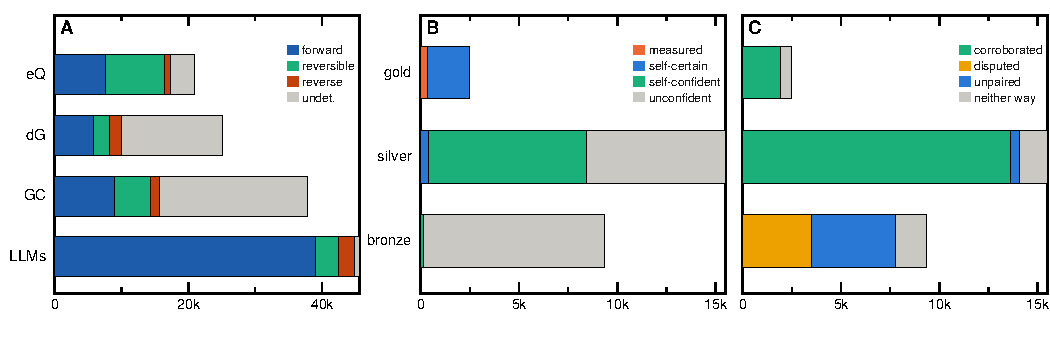
\includegraphics[width=\textwidth]{../figures/figure3_direction.pdf}}
\caption{
        \textbf{\DIFaddFL{Direction, agreement, and evidence.}} \DIFaddFL{(}\textbf{\DIFaddFL{A}}\DIFaddFL{) Direction assigned by each source independently: }\emph{\DIFaddFL{eQ}} \DIFaddFL{eQuilibrator, }\emph{\DIFaddFL{dG}} \DIFaddFL{dGPredictor, }\emph{\DIFaddFL{GC}} \DIFaddFL{group contribution, and }\emph{\DIFaddFL{LLMs}} \DIFaddFL{large language model ensemble that is not considered in evidence grading. Bar length is the number of reactions the source covers, facilitating comparison. (}\textbf{\DIFaddFL{B}}\DIFaddFL{) What each evidence grade rests on by the deciding source's own calibrated confidence, and (}\textbf{\DIFaddFL{C}}\DIFaddFL{) by what the other sources made of it. A reaction is }\emph{\DIFaddFL{self-certain}} \DIFaddFL{when the deciding source's calibrated probability of being within 2.0\,kcal\,mol$^{-1}$ of the true value ($p_{\text{ok}}$) is at $\ge0.90$, }\emph{\DIFaddFL{self-confident}} \DIFaddFL{is $0.7 \le p_{\text{ok}}\le 0.90$, and }\emph{\DIFaddFL{unconfident}} \DIFaddFL{is $p_{\text{ok}}\le 0.7$ (Supplementary Table~1).
    }} \label{fig:direction}
\end{figure*}

\DIFaddend %% Table 1 is the only table in the main text; the per-source breakdown that was
%% Table 3 in 2020 moves to Supplementary Table S1.
\subsection{Growth and coverage}\label{sec:results-growth}

The database has grown 34\% in  \DIFaddbegin \DIFadd{non-obsolete compounds and }\DIFaddend reactions since 2020,  driven mainly by MetaCyc and the BioCyc family.
Reaction growth is now split across three primary databases (Figure~\ref{fig:growth}B): MetaCyc carries 26,140 reactions of which 18,893 are  \DIFaddbegin \DIFadd{unique among the primary sources}\DIFaddend , KEGG 10,840 of which 5,291 are unique, and the newly-integrated Rhea 14,511 of which 8,210 are unique \DIFaddbegin \DIFadd{.
The completeness of reactions, meaning whether all involved compounds are structurally defined, differs among }\DIFaddend (Figure~\ref{fig:growth}C) : 90\%  \DIFaddbegin \DIFadd{for MetaCyc, }\DIFaddend 75\%  \DIFaddbegin \DIFadd{for KEGG, }\DIFaddend 65\%  \DIFaddbegin \DIFadd{for Rhea}\DIFaddend .
Overall structure coverage rose from 28,087 to 36,907 compounds ,  \DIFaddbegin \DIFadd{with the distribution of this new biochemistry described in Supplementary Methods~S5 and Supplementary Figure~S1}\DIFaddend .
\subsection{Structure curation}\label{sec:results-structure}

We built and ran our curation pipeline on all structures that would impact  \DIFaddbegin \DIFadd{a prioritized }\DIFaddend set of roughly 9,000 reactions used in  \DIFaddbegin \DIFadd{ModelSEED~\mbox{%DIFAUXCMD
\cite{henry2010,faria2023} }\hskip0pt%DIFAUXCMD
and PlantSEED~\mbox{%DIFAUXCMD
\cite{seaver2014,seaver2018}}\hskip0pt%DIFAUXCMD
}\DIFaddend .
This scope  \DIFaddbegin \DIFadd{is }\DIFaddend not a statement about how much of the database is usable .
The conflict pipeline resolved every previously conflicting compound in  \DIFaddbegin \DIFadd{a three-staged curation: i) historical formula were used to automatically resolve conflicts in mobile hydrogens, affecting 60 compounds and 550 reactions; ii) manual curation resolved conflicts in molecular structures, affecting 46 compounds and 59 reactions; and iii) where steps i-ii fail because of an absence in defensible source formula, reactions were added to a }\DIFaddend mass-balance exclusion registry where we fix an arbitrarily chosen formula \DIFaddbegin \DIFadd{, affecting 4 compounds and 61 reactions.
%DIF > % Figure 2 moved to M09 (2026-10) to pull it onto page 3; see M02's comment
%DIF > % on Figure 1 for the page-placement scheme this follows.
}\DIFaddend \subsection{Thermodynamics}\label{sec:results-thermo}

%% Counts measured 2026-09-08 from Biochemistry/reaction_*.json after the
%% Marvin 26.1 rebuild. Placeholders excluded per source: group contribution
%% dg = 1e7 (26,555 records); eQuilibrator sigma >= 2500 kcal/mol (3,386),
%% which is that source's refusal marker rather than an error bar.
The three predictors cover comparable fractions of the database and disagree substantially about how well they do it (Figure~\ref{fig:thermo}B). Uncertainty is reported on scales differing by more than an order of magnitude (Figure~\ref{fig:thermo}C):  \DIFaddbegin \DIFadd{median errors (}\DIFaddend kcal\,mol$^{-1}$ \DIFaddbegin \DIFadd{) of 0.62 for eQuilibrator, }\DIFaddend 10.83  for group contribution\DIFaddbegin \DIFadd{, }\DIFaddend and 17.57  for dGPredictor.

\paragraph{Calibrating the reported errors against measurement.} We use the experimental anchors to evaluate the error estimates.
For each source\DIFaddbegin \DIFadd{, }\DIFaddend we collect one held-out prediction per anchored reaction, together with the uncertainty that source reports for it, and divide the residual against the measured \drGo{} by that uncertainty.
Measured this way, eQuilibrator has a root mean square of 8.06 and a median of 2.27, with only 28.7\% of reactions within one reported standard deviation and 46.3\% within two, so  \DIFaddbegin \DIFadd{eQuilibrator }\DIFaddend understates its error.
Group contribution \DIFaddbegin \DIFadd{, by contrast, has }\DIFaddend a median of 0.32 and 73.6\% within one standard deviation, and dGPredictor  \DIFaddbegin \DIFadd{performs even better }\DIFaddend with a root mean square of 1.15 and 87.9\% within one  \DIFaddbegin \DIFadd{standard deviation.
%DIF >  A researcher choosing by smallest reported error would systematically choose the source that understates it, which is the argument against promoting any single source. 
}\DIFaddend The grading in the next section calibrates each source's confidence against measurement rather than taking its uncertainty at face value.

 \subsection{Direction assignment and evidence grading}\label{sec:results-direction}

%% All direction counts re-measured 2026-10-02 from Biochemistry/reaction_*.json
%% on the live (non-obsolete) population, after promoting the ab33a878 thermo
%% rerun's reaction_grades.tsv into thermo-evidence/reversibility (previously
%% unpromoted for 3 days) and re-running grade_thermo_sources.py --cv to drop
%% 5 reactions physically deleted by 3ac769c1 after ab33a878's snapshot.
%DIF > % Anchors: 363 distinct live reactions (801 stereo-exact records exist, but
%DIF > % 438 are obsolete duplicates of a live entry -- see S03 -- so the
%DIF > % predictors-alone re-grading below is computed over the 363 distinct ones).
%% The grade tiers are under active revision; the rates below are for the
%% scheme as it currently ships.
Each source now generates its own prediction for the direction each reaction proceeds, and the three sources differ more in what they will commit to than in what they say (Figure~\ref{fig:direction}A).
eQuilibrator resolves 97.4\% of the reactions it covers, group contribution 59.7\%\DIFaddbegin \DIFadd{, }\DIFaddend and dGPredictor 40.1\%.
Across the database, 24,594 reactions receive a direction or a positive statement of reversibility from at least one source and 23,790 receive none.

\paragraph{eQuilibrator vs dGPredictor} dGPredictor is able to generate a predicted energy for more reactions ($\sim25,100$, against eQuilibrator's $\sim17,900$) and converts the least of that coverage into a usable reaction direction.
For a typical  \DIFaddbegin \DIFadd{reaction, }\DIFaddend the error bar \DIFaddbegin \DIFadd{from dGPredictor }\DIFaddend alone exceeds the decision threshold in the reversibility index, so 59.9\% of its reactions are returned undetermined  \DIFaddbegin \DIFadd{versus }\DIFaddend 2.6\%  \DIFaddbegin \DIFadd{from eQuilibrator.
These sources agree 94.8\% when they }\DIFaddend commit to a direction ,  \DIFaddbegin \DIFadd{although eQuilibrator provides more unique predictions (}\DIFaddend 11,237 \DIFaddbegin \DIFadd{) than dGPredictor provides (3,877) because dGPredictor often abstains rather than contradicting}\DIFaddend .

\paragraph{Grading.} Of 27,338 graded reactions, 4,073 are gold, 14,475 silver and 8,790 bronze (Figure~\ref{fig:direction}B,C; see classification scheme in Supplementary Methods~S3).
The tiers separate on what supports them: gold is 91\% self-certain and 85\% corroborated  while bronze is 99\% unconfident \DIFaddbegin \DIFadd{, either uncorroborated }\DIFaddend (48\%)  \DIFaddbegin \DIFadd{or contradicted }\DIFaddend (29\%) \DIFaddbegin \DIFadd{by other sources}\DIFaddend .
Because a measured reaction is always graded gold, the grades must be recomputed with openTECR withheld before they can be tested against it.
Re-graded on the predictors alone, the  \DIFaddbegin \DIFadd{363 distinct anchored reactions split into 172 gold, 186 silver and 5 bronze.
The gold and silver reactions fall }\DIFaddend within 2\,kcal\,mol$^{-1}$ of measurement  \DIFaddbegin \DIFadd{93.0\% and 89.2\% of the time }\DIFaddend (Supplementary Methods~S3) \DIFaddbegin \DIFadd{, hence we recommend these tiers }\DIFaddend for inclusion in a metabolic model  and reserve bronze for review rather than use \DIFaddbegin \DIFadd{in models}\DIFaddend .

\paragraph{Recommendation.}  \DIFaddbegin \DIFadd{We recommend the consensus among sources, but when sources disagree on }\DIFaddend reaction direction,  \DIFaddbegin \DIFadd{we prioritize eQuilibrator followed by dGPredictor and then }\DIFaddend group contribution.
\DIFaddbegin \DIFadd{Following this tiered approach, }\DIFaddend eQuilibrator supplies 16,985 recommended reaction directions, dGPredictor \DIFaddbegin \DIFadd{provides }\DIFaddend 7,935\DIFaddbegin \DIFadd{, }\DIFaddend and group contribution \DIFaddbegin \DIFadd{provides }\DIFaddend 2,055 \DIFaddbegin \DIFadd{, the source for each recommendation being recorded.
}\DIFaddend 

\DIFaddbegin \subsection{\DIFadd{Ensemble LLMs predictions}}\label{sec:llm-grading-rslts}
\DIFadd{The ensemble generated calls for $\sim46,000$ reactions (Figure~\ref{fig:direction}) and $\sim23,000$ directions for reactions that no thermodynamic source committed on.
However, 85\% of its calls are simply the direction the equation is written in (Supplementary Methods~S4), so we exclude these calls from evidence grading and report them as a separate, clearly-labelled layer.
Neither the thermodynamics nor the ensemble approaches capture the context of metabolic pathways that can drive a reaction against its own standard-state energy as metabolite concentrations shift downstream~\mbox{%DIFAUXCMD
\cite{noor2014}}\hskip0pt%DIFAUXCMD
.
}\DIFaddend %% Consolidates the former results_{atom_mapping,reaction_similarity,
%% connectivity_ontology} sections.
\subsection{Atom mapping}\label{sec:results-mapping}

Atom mappings are published for 26,242 reactions, 54\% of the database: 19,809 clean, and 6,433 that required salvage (which are tagged). As the mappings can be used to span a metabolic reconstruction, reactions needing one repair are likely to carry others.


 \section{Discussion}

Unlike the 2020 release, this update adopts a multi-source  \DIFaddbegin \DIFadd{approach }\DIFaddend rather than promoting a single thermodynamic value, publishing four sources  \DIFaddbegin \DIFadd{that each have }\DIFaddend their own uncertainty and estimated direction,  \DIFaddbegin \DIFadd{to capture source diversity}\DIFaddend .
Grading against experiment enables us to validate the approach: A researcher can take the highest-graded source and  \DIFaddbegin \DIFadd{know }\DIFaddend what the grade means.
 \DIFaddbegin \DIFadd{As this is a generalized reference database, we intentionally exclude organism-specific data; a choice affecting transport reactions and metabolic reconstruction that we discuss in Supplementary Methods~S6.
A current limitation is that }\DIFaddend roughly half the database  \DIFaddbegin \DIFadd{lacks thermodynamic values, constrained by missing or incomplete chemical structures.
For the remaining reactions, by explicitly reporting discrepancies among thermodynamic }\DIFaddend sources, we  \DIFaddbegin \DIFadd{aim to better serve researchers who rely on standardized biochemistry for }\DIFaddend genome-scale reconstruction, flux analysis, pathway design \DIFaddbegin \DIFadd{, and predictive modeling.
}

\DIFaddend \section{Data availability}

The ModelSEED Biochemistry Database is available at \url{https://github.com/ModelSEED/ModelSEEDDatabase} under the Creative Commons Attribution License, as versioned flat files and JSON, and archived at Zenodo (\url{https://doi.org/10.5281/zenodo.22782602}). Data directly derived from KEGG and MetaCyc remain subject to the licences of those resources. It is also queryable through a Solr endpoint and browsable at \modelseedurl. Released structures, thermodynamic values with per-source uncertainty, evidence grades, atom mappings and the low-confidence reaction flags are all in that repository. The scripts that regenerate every published value, including the eQuilibrator cache rebuild, are under \file{Scripts/Thermodynamics/}.

%% Supplied by Robert Giessmann (2026-09-14), his own wording. Only change:
%% ``wants to acknowledge'' -> ``acknowledges'' for journal register. NAR's
%% Article structure list places Acknowledgements before Author Contributions.
\section{Acknowledgements} R.T.G.\ acknowledges all the hard-working individuals who contributed their time voluntarily to transcribe and check the myriad of numbers and text to create the re-curated openTECR v1.0. The full list of contributors can be found at \url{https://github.com/opentecr}.

%% DRAFT for circulation, not agreed. Role assignment follows Sam's steer of
%% 2026-09-10: Sam lead throughout; Henry conceptualization plus funding and
%% supervision; Freiburger, Faria, Setlur and Taylor major, each supplying part
%% of the resources the release was assembled from; Edirisinghe and Liu minor.
%% External groups are credited for the tool or dataset they contributed.
%% Degrees (lead/equal/supporting) are CRediT's own qualifiers and carry the
%% major/minor distinction without ranking people. Every author must confirm
%% their own line: NAR requires editor approval to change roles after submission.
\section{Author contributions} Contributions follow the CRediT taxonomy. S.M.D.S.: conceptualization, methodology, software, formal analysis, data curation, visualization, writing -- original draft, project administration. C.S.H.: conceptualization, funding acquisition, supervision. A.F., J.P.F., V.S.\ and C.T.: resources, data curation, investigation; J.P.F.\ also writing -- original draft. J.N.E.\ and F.L.: resources, software (supporting). R.T.G.: the openTECR re-curation of the experimental measurements. E.N.\ and M.E.B.: eQuilibrator. V.U., M.A.\ and C.D.M.: dGPredictor. S.H.\ and Z.N.: atom mapping. A.P.A., R.W.C.\ and E.M.W.-C.: funding acquisition, supervision. All authors reviewed the manuscript.

\section{Funding}
%% Sam's wording, 2026-09-07. BRAVE's identifier is as he supplied it.
%%
%% KBase is cited with its FOUR EXTERNAL DOE AWARD NUMBERS, taken from the
%% funding acknowledgement of the most recent KBase paper. An earlier draft of
%% this section used PRJ1003559, which appears in cv.md and 19 times in the
%% mail archive -- but that is an INTERNAL Argonne cost code
%% ("PRJ1003559 66370 Kbase Pred Bio Environ"), not a DOE award number, and it
%% does not belong in a funding statement. Do not reinstate it.
%%
%% DE-AC02-06CH11357 deliberately appears TWICE: once as Argonne's operating
%% contract for this work, and once within KBase's own award list, where it is
%% Argonne's share of the KBase award. That is how KBase states it.
This work was supported by the U.S. Department of Energy, Office of Science, Biological and Environmental Research, under Argonne National Laboratory contract DE-AC02-06CH11357. We specifically acknowledge support from the BRAVE FWP (DOE-112-VAM-PRJ1011481). The DOE Systems Biology Knowledgebase (KBase) is funded by the U.S. Department of Energy, Office of Science, Office of Biological and Environmental Research, under Award Numbers DE-AC02-05CH11231, DE-AC02-06CH11357, DE-AC05-00OR22725, and DE-SC0012704.

\section{Conflict of interest} None declared.

\section{Notice of copyright} The submitted manuscript has been created by UChicago Argonne, LLC, Operator of Argonne National Laboratory (``Argonne''). Argonne, a U.S. Department of Energy Office of Science laboratory, is operated under Contract No.~DE-AC02-06CH11357. The U.S. Government retains for itself, and others acting on its behalf, a paid-up nonexclusive, irrevocable worldwide license in said article to reproduce, prepare derivative works, distribute copies to the public, and perform publicly and display publicly, by or on behalf of the Government. The Department of Energy will provide public access to these results of federally sponsored research in accordance with the DOE Public Access Plan. \url{http://energy.gov/downloads/doe-public-access-plan}


\bibliographystyle{nar}
\begin{thebibliography}{10}

\bibitem{seaver2020}
Seaver, S. M.~D., Liu, F., Zhang, Q., et al. (2021)
The {ModelSEED} Biochemistry Database for the integration of metabolic
  annotations and the reconstruction, comparison and analysis of metabolic
  models for plants, fungi and microbes.
{\em Nucleic Acids Research,} {\bf 49}(D1), D575--D588.

\bibitem{gemsembler2025}
Matveishina, E.~K., Bartmanski, B.~J., Benito-Vaquerizo, S., and
  Zimmermann-Kogadeeva, M. (2025)
{GEMsembler}: consensus model assembly and structural comparison of
  genome-scale metabolic models across tools improve functional performance.
{\em mSystems,} {\bf 10}(10), e0057425.

\bibitem{yeast9}
Zhang, C., S{\'a}nchez, B.~J., Li, F., et al. (2024)
{Yeast9}: a consensus genome-scale metabolic model for {S. cerevisiae} curated
  by the community.
{\em Molecular Systems Biology,} {\bf 20}(10), 1134--1150.

\bibitem{caspi2020}
Caspi, R., Billington, R., Keseler, I.~M., et al. (2020)
The {MetaCyc} database of metabolic pathways and enzymes --- a 2019 update.
{\em Nucleic Acids Research,} {\bf 48}(D1), D445--D453.

\bibitem{bansal2022}
Bansal, P., Morgat, A., Axelsen, K.~B., et al. (2022)
{Rhea}, the reaction knowledgebase in 2022.
{\em Nucleic Acids Research,} {\bf 50}(D1), D693--D700.

\bibitem{hastings2016}
Hastings, J., Owen, G., Dekker, A., et al. (2016)
{ChEBI} in 2016: Improved services and an expanding collection of metabolites.
{\em Nucleic Acids Research,} {\bf 44}(D1), D1214--D1219.

\bibitem{flamholz2012}
Flamholz, A., Noor, E., Bar-Even, A., and Milo, R. (2012)
{eQuilibrator} --- the biochemical thermodynamics calculator.
{\em Nucleic Acids Research,} {\bf 40}(D1), D770--D775.

\bibitem{jankowski2008}
Jankowski, M.~D., Henry, C.~S., Broadbelt, L.~J., and Hatzimanikatis, V. (2008)
Group contribution method for thermodynamic analysis of complex metabolic
  networks.
{\em Biophysical Journal,} {\bf 95}(3), 1487--1499.

\bibitem{beber2022}
Beber, M.~E., Gollub, M.~G., Mozaffari, D., et al. (2022)
{eQuilibrator} 3.0: a database solution for thermodynamic constant estimation.
{\em Nucleic Acids Research,} {\bf 50}(D1), D603--D609.

\bibitem{wang2021}
Wang, L., Upadhyay, V., and Maranas, C.~D. (2021)
{dGPredictor}: Automated fragmentation method for metabolic reaction free
  energy prediction and de novo pathway design.
{\em PLOS Computational Biology,} {\bf 17}(9), e1009448.

\bibitem{alberty2003}
Alberty, R.~A. (2003)
Thermodynamics of Biochemical Reactions,
Wiley-Interscience, Hoboken, NJ.

\bibitem{marvin}
{ChemAxon}
{Marvin} 26.1.
\url{https://www.chemaxon.com} (2026)
Chemical structure and p$K_\mathrm{a}$ prediction toolkit.

\bibitem{pan2021}
Pan, X., Wang, H., Li, C., Zhang, J. Z.~H., and Ji, C. (2021)
{MolGpKa}: A Web Server for Small Molecule $\mathrm{p}K_a$ Prediction Using a
  Graph-Convolutional Neural Network.
{\em Journal of Chemical Information and Modeling,} {\bf 61}(7), 3159--3165.

\bibitem{goldberg2004}
Goldberg, R.~N., Tewari, Y.~B., and Bhat, T.~N. (2004)
Thermodynamics of enzyme-catalyzed reactions --- a database for quantitative
  biochemistry.
{\em Bioinformatics,} {\bf 20}(16), 2874--2877.

\bibitem{noor2012}
Noor, E., Bar-Even, A., Flamholz, A., et al. (2012)
An integrated open framework for thermodynamics of reactions that combines
  accuracy and coverage.
{\em Bioinformatics,} {\bf 28}(15), 2037--2044.

\bibitem{huss2022}
Hu{\ss}, S., Judd, R.~S., Koper, K., Maeda, H.~A., and Nikoloski, Z. (2022)
An automated workflow that generates atom mappings for large-scale metabolic
  models and its application to {A}rabidopsis thaliana.
{\em The Plant Journal,} {\bf 111}(5), 1486--1500.

\bibitem{rahman2016}
Rahman, S.~A., Torrance, G., Baldacci, L., et al. (2016)
Reaction Decoder Tool ({RDT}): extracting features from chemical reactions.
{\em Bioinformatics,} {\bf 32}(13), 2065--2066.

\bibitem{henry2010}
Henry, C.~S., DeJongh, M., Best, A.~A., Frybarger, P.~M., Linsay, B., and
  Stevens, R.~L. (2010)
High-throughput generation, optimization and analysis of genome-scale metabolic
  models.
{\em Nature Biotechnology,} {\bf 28}(9), 977--982.

\bibitem{faria2023}
Faria, J.~P., Liu, F., Edirisinghe, J.~N., Gupta, N., Seaver, S. M.~D.,
  Freiburger, A.~P., Setlur, V., Zhang, Q., Weisenhorn, P., Conrad, N.,
  Zarecki, R., Song, H.-S., DeJongh, M., Best, A.~A., Cottingham, R.~W., Arkin,
  A.~P., and Henry, C.~S. (2023)
{ModelSEED} v2: High-throughput genome-scale metabolic model reconstruction
  with enhanced energy biosynthesis pathway prediction.
{\em bioRxiv,}.

\bibitem{seaver2014}
Seaver, S. M.~D., Gerdes, S., Frelin, O., Lerma-Ortiz, C., Bradbury, L. M.~T.,
  Zallot, R., Hasnain, G., Niehaus, T.~D., El~Yacoubi, B., Pasternak, S.,
  Olson, R., Pusch, G., Overbeek, R., Stevens, R., de~Cr\'ecy-Lagard, V., Ware,
  D., Hanson, A.~D., and Henry, C.~S. (2014)
High-throughput comparison, functional annotation, and metabolic modeling of
  plant genomes using the {PlantSEED} resource.
{\em Proceedings of the National Academy of Sciences,} {\bf 111}(26),
  9645--9650.

\bibitem{seaver2018}
Seaver, S. M.~D., Lerma-Ortiz, C., Conrad, N., Mikaili, A., Sreedasyam, A.,
  Hanson, A.~D., and Henry, C.~S. (2018)
{PlantSEED} enables automated annotation and reconstruction of plant primary
  metabolism with improved compartmentalization and comparative consistency.
{\em The Plant Journal,} {\bf 95}(6), 1102--1113.

\bibitem{noor2014}
Noor, E., Bar-Even, A., Flamholz, A., et al. (2014)
Pathway thermodynamics highlights kinetic obstacles in central metabolism.
{\em PLoS Computational Biology,} {\bf 10}(2), e1003483.

\end{thebibliography}

\end{document}
